%%This is a very basic article template.
%%There is just one section and two subsections.
\documentclass[11pt, a4paper, openany]{article}

\usepackage[top=1.25in, bottom=1.25in, left=1.25in, right=1.25in]{geometry}

\usepackage[english]{babel}
\usepackage[utf8]{inputenc}
\usepackage[T1]{fontenc}

%\setlength\textwidth{16cm}
%\setlength\oddsidemargin{1cm} 
%%\setlength\oddsidemargin{1cm} 
%%\setlength\evensidemargin{1cm}

\usepackage{IDA}

\usepackage[pdftex]{graphicx}

\graphicspath{{./img/pdf/}{./img/png/}}

\usepackage{pdfpages}
\pdfoutput=1
\pdfcompresslevel=9 
\DeclareGraphicsExtensions{.pdf,.jpg,.png}

% settings
\clubpenalty = 10000
\widowpenalty = 10000
\displaywidowpenalty = 10000
\sloppy % allow wider spaces to avoid lines going too wide

\usepackage[most]{tcolorbox}
\usepackage{enumitem}
\usepackage{graphicx}
\usepackage{subcaption}
\usepackage[]{placeins}
\usepackage{textcomp}
\usepackage{amsthm}
\newtheorem{assumption}{Assumption}
\newtheorem{theorem}{Theorem}
\newtheorem{lemma}{Lemma}
\newtheorem{definition}{Definition}
\newtheorem{example}{Example}
\usepackage{amsmath}
\usepackage{amssymb}
\usepackage{xcolor}
\usepackage[bottom]{footmisc}
\usepackage[nolist]{acronym}
% lastly load colour hyperref
\usepackage[pdftex,plainpages=true,pdfpagelabels,colorlinks,pdfusetitle]{hyperref}
% Hyperref Einstellungen
\hypersetup{
 pdfkeywords={...},
% backref=true,
% pagebackref=true,
% hyperfigures,
% hyperindex,
 colorlinks,
 pdfpagemode=UseOutlines,
 bookmarksopen,
 bookmarksopenlevel=1,
 bookmarksnumbered,
% bookmarksdepth=5, %this only works in a current version of hyperref
 pageanchor,
 plainpages=true,
 urlcolor=black,
 menucolor=black,
 citecolor=black,
 anchorcolor=black,
 filecolor=black,
 linkcolor=black,
 colorlinks=true
}
\usepackage{booktabs}
%\usepackage{tabularx} 
\usepackage{multirow}
\usepackage{array}
\newcolumntype{L}[1]{>{\raggedright\let\newline\\\arraybackslash\hspace{0pt}}m{#1}}
\newcolumntype{C}[1]{>{\centering\let\newline\\\arraybackslash\hspace{0pt}}m{#1}}
\newcolumntype{R}[1]{>{\raggedleft\let\newline\\\arraybackslash\hspace{0pt}}m{#1}}
\usepackage{rotating}
\usepackage{chngpage} %allows temporary cheating with page margins
\usepackage{layouts}
%\usepackage[format=plain, justification=centering,singlelinecheck=false]{caption}
\usepackage[justification=centering,singlelinecheck=false]{caption}
% \usepackage{algorithm}
% \usepackage[noend]{algorithmic}
%\renewcommand{\algorithmicrequire}{\textbf{Input:}}
\usepackage{listings}
\usepackage{etoolbox}
%\usepackage{subcaption}
\usepackage{tikzsymbols}
\usepackage{tcolorbox}
%\usepackage[justification=centering]{caption}
\usepackage{wasysym}
\usepackage{hyperref}
\usepackage[normalem]{ulem}
\usepackage{here}
\usepackage{tikz}
\usetikzlibrary{svg.path}

\usepackage[justification=raggedright]{caption}
\usepackage{xargs}
\usepackage{pdfpages}
\newcommandx{\platform}{\mathcal{P}}
\newcommandx{\ResourceSet}{\mathcal{R}}
\newcommandx{\Resource}{R}
\newcommandx{\pResource}{{R}_p}
\newcommandx{\pResourceSet}{\mathcal{R}_p}
\newcommandx{\cResource}{{R}_c}
\newcommandx{\cResourceSet}{\mathcal{R}_c}
\newcommandx{\linkSet}{\mathcal{E}}

\newcommandx{\app}{\mathcal{A}}
\newcommandx{\dependSet}{\mathcal{D}}
\newcommandx{\taskSet}{\mathcal{T}}
\newcommandx{\task}[2][1=i,2=c]{\tau^{#2}_{#1}}
\newcommandx{\taskStd}[1][1=i]{\tau_{#1}}
\newcommandx{\job}[3][1=i,2=j,3=c]{\tau^{#3}_{#1}(#2)}
\newcommandx{\jobStd}[2][1=i,2=j]{\tau_{#1}(#2)}
\newcommandx{\re}[2]{\rho_{#1}(#2)}
\newcommandx{\cec}{C}
\newcommandx{\jobSeq}{j_1,j_2,\ldots,j_n}
\newcommandx{\jobSeqShort}{j_1,\ldots,j_n}
\newcommandx{\chain}{\cec^{et}}
\newcommandx{\ttChain}{\cec^{tt}}
\newcommandx{\etChain}{\cec^{et}}
\newcommandx{\letChain}{\cec^{let}}
%
%deadline
\newcommandx{\deadline}[1]{d_{\task[#1]}}
\newcommandx{\deadlineStd}[1]{d_{\taskStd[#1]}}
\newcommandx{\eteDeadline}[1][1=\cec]{d^{e2e}_{#1}}
%
%
%execution times
\newcommandx{\bcet}[1]{BCET_{\task[#1]}}
\newcommandx{\bcetStd}[1]{BCET_{\taskStd[#1]}}
\newcommandx{\wcet}[1]{WCET_{\task[#1]}}
\newcommandx{\wcetStd}[1]{WCET_{\taskStd[#1]}}
\newcommandx{\Let}[1]{LET_{\task[#1]}}
\newcommandx{\LetStd}[1]{LET_{\taskStd[#1]}}
%
%%response times
\newcommandx{\bcrt}[1]{BCRT_{\task[#1]}}
\newcommandx{\bcrtStd}[1]{BCRT_{\taskStd[#1]}}
\newcommandx{\wcrt}[1]{WCRT_{\task[#1]}}
\newcommandx{\wcrtStd}[1]{WCRT_{\taskStd[#1]}}
%robustness
\newcommandx{\disturb}[1][1=i]{\Delta \wcrt{#1}}
\newcommandx{\disturbLet}[1]{\Delta \Let{#1}}
\newcommandx{\wcrtPrime}[1][1=i]{\wcrt{#1}'}
\newcommandx{\LetPrime}[1][1=i]{\Let{#1}'}
\newcommandx{\margin}[2][2=\cec]{RM^{#2}(#1)}
\newcommandx{\marginAll}[2][2=\cec]{RM(#1)}
\newcommandx{\jobs}[1]{\mathcal{J}_{HP,#1}}
%
%%activation patterns
\newcommandx{\offset}[1]{\Phi_{\task[#1]}}
\newcommandx{\offsetStd}[1]{\Phi_{\taskStd[#1]}}
\newcommandx{\period}[1]{P_{\task[#1]}}
\newcommandx{\periodStd}[1]{P_{\taskStd[#1]}}
\newcommandx{\deltaMin}[2][2=n]{\underline{\delta}_{\task[#1]}(#2)}
\newcommandx{\deltaMinStd}[2][2=n]{\underline{\delta}_{#1}(#2)}
\newcommandx{\deltaMax}[2][2=n]{\overline{\delta}_{\task[#1]}(#2)}
\newcommandx{\deltaMaxStd}[2][2=n]{\overline{\delta}_{#1}(#2)}

%tree
\newcommandx{\tree}{\mathcal{T}}

%intervals
\newcommandx{\readMin}[1]{\underline{R}\left(#1\right)}
\newcommandx{\readMax}[1]{\overline{R}\left(#1\right)}
\newcommandx{\readInt}[1]{RI\left(#1\right)}
\newcommandx{\dataMin}[1]{\underline{D}\left(#1\right)}
\newcommandx{\dataMax}[1]{\overline{D}\left(#1\right)}
\newcommandx{\dataInt}[1]{DI\left(#1\right)}

%latencies
\newcommandx{\lat}[1]{Lat(#1)}
\newcommandx{\latMax}[1][1=\cec]{\overline{Lat}(#1)}
%
\newcommandx{\tlat}[1]{TLat(#1)}
\newcommandx{\TtTtTlat}{TLat(\ttChain, \ttChain)}
\newcommandx{\TtLetTlat}{TLat(\ttChain, \letChain)}
\newcommandx{\TtEtTlat}{TLat(\ttChain, \etChain)}
\newcommandx{\LetTtTlat}{TLat(\letChain, \ttChain)}
\newcommandx{\LetLetTlat}{TLat(\letChain, \letChain)}
\newcommandx{\LetEtTlat}{TLat(\letChain, \etChain)}
\newcommandx{\EtTtTlat}{TLat(\etChain, \ttChain)}
\newcommandx{\EtLetTlat}{TLat(\etChain, \letChain)}
\newcommandx{\EtEtTlat}{TLat(\etChain, \etChain)}
%
\newcommandx{\tlatMax}[1]{\overline{TLat}(#1)}




% Some useful commands and a notation package
% Thy to Moritz :-)
\newcommand{\chapref}[1]{chapter~\ref{#1}}
\newcommand{\secref}[1]{Section~\ref{#1}}
\newcommand{\figref}[1]{figure~\ref{#1}}
\newcommand{\FigRef}[1]{Figure~\ref{#1}}
\newcommand{\equaref}[1]{(\ref{#1})}
\newcommand{\algref}[1]{algorithm~\ref{#1}}
\newcommand{\tabref}[1]{table~\ref{#1}}
\newcommand{\defref}[1]{definition~\ref{#1}}
\newcommand{\theoremref}[1]{theorem~\ref{#1}}
\newcommand{\lemmaref}[1]{lemma~\ref{#1}}
\newcommand{\corollaryref}[1]{corollary~\ref{#1}}
\newcommand{\appref}[1]{Appendix~\ref{#1}}

\newcommand{\Chapref}[1]{Chapter~\ref{#1}}
\newcommand{\Secref}[1]{Section~\ref{#1}}
\newcommand{\Figref}[1]{Figure~\ref{#1}}
\newcommand{\Equaref}[1]{(Equation~\ref{#1})}
\newcommand{\Algref}[1]{Algorithm~\ref{#1}}
\newcommand{\Tabref}[1]{Table~\ref{#1}}
\newcommand{\Defref}[1]{Definition~\ref{#1}}
\newcommand{\Theoremref}[1]{Theorem~\ref{#1}}
\newcommand{\Lemmaref}[1]{Lemma~\ref{#1}}
\newcommand{\Corollaryref}[1]{Corollary~\ref{#1}}
\newcommand{\Appref}[1]{Appendix~\ref{#1}}
\newcommand{\Lstref}[1]{Lst.~\ref{#1}}
\newcommand{\Code}[1]{\texttt{#1}}
\newcommand{\ucos}{$\mu$C/OS-II~}
\newcommand{\citeme}{\textbf{\textcolor{red}{CITEME}}}
%\newcommandx{\platform}{\mathcal{P}}
\newcommandx{\ResourceSet}{\mathcal{R}}
\newcommandx{\Resource}{R}
\newcommandx{\pResource}{{R}_p}
\newcommandx{\pResourceSet}{\mathcal{R}_p}
\newcommandx{\cResource}{{R}_c}
\newcommandx{\cResourceSet}{\mathcal{R}_c}
\newcommandx{\linkSet}{\mathcal{E}}

\newcommandx{\app}{\mathcal{A}}
\newcommandx{\dependSet}{\mathcal{D}}
\newcommandx{\taskSet}{\mathcal{T}}
\newcommandx{\task}[2][1=i,2=c]{\tau^{#2}_{#1}}
\newcommandx{\taskStd}[1][1=i]{\tau_{#1}}
\newcommandx{\job}[3][1=i,2=j,3=c]{\tau^{#3}_{#1}(#2)}
\newcommandx{\jobStd}[2][1=i,2=j]{\tau_{#1}(#2)}
\newcommandx{\re}[2]{\rho_{#1}(#2)}
\newcommandx{\cec}{C}
\newcommandx{\jobSeq}{j_1,j_2,\ldots,j_n}
\newcommandx{\jobSeqShort}{j_1,\ldots,j_n}
\newcommandx{\chain}{\cec^{et}}
\newcommandx{\ttChain}{\cec^{tt}}
\newcommandx{\etChain}{\cec^{et}}
\newcommandx{\letChain}{\cec^{let}}
%
%deadline
\newcommandx{\deadline}[1]{d_{\task[#1]}}
\newcommandx{\deadlineStd}[1]{d_{\taskStd[#1]}}
\newcommandx{\eteDeadline}[1][1=\cec]{d^{e2e}_{#1}}
%
%
%execution times
\newcommandx{\bcet}[1]{BCET_{\task[#1]}}
\newcommandx{\bcetStd}[1]{BCET_{\taskStd[#1]}}
\newcommandx{\wcet}[1]{WCET_{\task[#1]}}
\newcommandx{\wcetStd}[1]{WCET_{\taskStd[#1]}}
\newcommandx{\Let}[1]{LET_{\task[#1]}}
\newcommandx{\LetStd}[1]{LET_{\taskStd[#1]}}
%
%%response times
\newcommandx{\bcrt}[1]{BCRT_{\task[#1]}}
\newcommandx{\bcrtStd}[1]{BCRT_{\taskStd[#1]}}
\newcommandx{\wcrt}[1]{WCRT_{\task[#1]}}
\newcommandx{\wcrtStd}[1]{WCRT_{\taskStd[#1]}}
%robustness
\newcommandx{\disturb}[1][1=i]{\Delta \wcrt{#1}}
\newcommandx{\disturbLet}[1]{\Delta \Let{#1}}
\newcommandx{\wcrtPrime}[1][1=i]{\wcrt{#1}'}
\newcommandx{\LetPrime}[1][1=i]{\Let{#1}'}
\newcommandx{\margin}[2][2=\cec]{RM^{#2}(#1)}
\newcommandx{\marginAll}[2][2=\cec]{RM(#1)}
\newcommandx{\jobs}[1]{\mathcal{J}_{HP,#1}}
%
%%activation patterns
\newcommandx{\offset}[1]{\Phi_{\task[#1]}}
\newcommandx{\offsetStd}[1]{\Phi_{\taskStd[#1]}}
\newcommandx{\period}[1]{P_{\task[#1]}}
\newcommandx{\periodStd}[1]{P_{\taskStd[#1]}}
\newcommandx{\deltaMin}[2][2=n]{\underline{\delta}_{\task[#1]}(#2)}
\newcommandx{\deltaMinStd}[2][2=n]{\underline{\delta}_{#1}(#2)}
\newcommandx{\deltaMax}[2][2=n]{\overline{\delta}_{\task[#1]}(#2)}
\newcommandx{\deltaMaxStd}[2][2=n]{\overline{\delta}_{#1}(#2)}

%tree
\newcommandx{\tree}{\mathcal{T}}

%intervals
\newcommandx{\readMin}[1]{\underline{R}\left(#1\right)}
\newcommandx{\readMax}[1]{\overline{R}\left(#1\right)}
\newcommandx{\readInt}[1]{RI\left(#1\right)}
\newcommandx{\dataMin}[1]{\underline{D}\left(#1\right)}
\newcommandx{\dataMax}[1]{\overline{D}\left(#1\right)}
\newcommandx{\dataInt}[1]{DI\left(#1\right)}

%latencies
\newcommandx{\lat}[1]{Lat(#1)}
\newcommandx{\latMax}[1][1=\cec]{\overline{Lat}(#1)}
%
\newcommandx{\tlat}[1]{TLat(#1)}
\newcommandx{\TtTtTlat}{TLat(\ttChain, \ttChain)}
\newcommandx{\TtLetTlat}{TLat(\ttChain, \letChain)}
\newcommandx{\TtEtTlat}{TLat(\ttChain, \etChain)}
\newcommandx{\LetTtTlat}{TLat(\letChain, \ttChain)}
\newcommandx{\LetLetTlat}{TLat(\letChain, \letChain)}
\newcommandx{\LetEtTlat}{TLat(\letChain, \etChain)}
\newcommandx{\EtTtTlat}{TLat(\etChain, \ttChain)}
\newcommandx{\EtLetTlat}{TLat(\etChain, \letChain)}
\newcommandx{\EtEtTlat}{TLat(\etChain, \etChain)}
%
\newcommandx{\tlatMax}[1]{\overline{TLat}(#1)}




\usepackage{xspace}
\newcommand{\Tool}{
\textbf{\textsc{\rmfamily{Toro}}}\xspace}

\definecolor{dkgreen}{rgb}{0,0.6,0}
\definecolor{gray}{rgb}{0.5,0.5,0.5}
\definecolor{mauve}{rgb}{0.58,0,0.82}

\lstset{frame=tb,
  language=C,
  aboveskip=3mm,
  belowskip=-1mm,
  showstringspaces=false,
  columns=flexible,
  basicstyle={\small\ttfamily},
  numbers=none,
  numberstyle=\tiny\color{gray},
  keywordstyle=\color{blue},
  commentstyle=\color{dkgreen},
  stringstyle=\color{mauve},
  breaklines=true,
  breakatwhitespace=true,
  tabsize=3
}

\newcommand{\deliverable}{Robuste Wirkketten}
\newcommand{\shorttitle}{Abschlussbericht AP3}

\setlength\parindent{0pt}

\begin{document} 

\begin{acronym}[ECU]
\acro{spp}[SPP]{static priority preemptive}
\acro{spnp}[SPNP]{static priority non-preemptive}
\acro{wcrt}[WCRT]{maximale Antwortzeit}
\end{acronym}


% Modifiy font sizes, requires \usepackage{etoolbox} in packages.tex
\newcommand{\EqSize}{\small}			% Equations and Align
\newcommand{\AlgSize}{\small}			% Algorithm
\newcommand{\LstSize}{\scriptsize}			% Source code listing
\preto\align{\par\nobreak\EqSize\noindent}
\preto\equation{\par\nobreak\EqSize\noindent}
\preto\algorithmic{\par\nobreak\AlgSize\noindent}
%\preto\lstlisting{\par\nobreak\noident}

\begin{titlepage}
\pagestyle{plain}
\pagenumbering{Alph}
% \includegraphics[width=5cm]{img/iTUBS}\\[3cm] 

\title{\Tool: \\
\LARGE{A TOol to evaluate the RObustness}\\ 
\LARGE{of cause-effect chains}.}
\author{
Leonie Köhler, M.Sc.\\%
Nikolas Brendes, B.Sc. \\
Prof. Dr.-Ing. Rolf Ernst}
\date{Version 1.0}
\maketitle 
\thispagestyle{empty}


\begin{flushright}

\Large\textbf{Abschlussbericht AP3}
\\[1cm]
\large
iTUBS \\ Braunschweig 
\end{flushright} 

%\vspace{5cm}
%\begin{abstract}
%Abstract goes here
%\end{abstract}

\end{titlepage}

\pagenumbering{roman}
\pagestyle{plain}

\tableofcontents
\clearpage
%\newpage
%\listoffigures
%\listoftables
%\newpage
\clearpage
\pagestyle{fancyplain}
\pagenumbering{arabic}



%%% CONTENT:
\section{Deliverables of AP 3}
\begin{itemize}
	\item \Tool, TOol to evaluate the RObustness of cause-effect chains
	\item Documentation
	\item PowerPoint Presentation
	\item \emph{Additionally}\\
	Joint conference paper, submission to ECRTS'20 planned
\end{itemize}

\newpage

\section{Introduction}
Control applications in automotive software systems often contain time-critical cause-effect chains.  
A time-critical chain typically includes the reading of sensor data, their processing and finally the control of actuators.  
Satisfying specified end-to-end deadlines of cause-effect  chains serves to ensure correct system behavior and can also increase driving comfort.
From an implementation point of view, a cause-effect chain consists of communicating tasks that are distributed among various system components. 
\smallskip

Designing a software application in such a way that all end-to-end deadlines of cause-effect chains are satisfied, even in the worst case, is challenging. 
Since software applications are regularly extended, it is another central concern to guarantee end-to-end deadlines in case of software updates without having to carry out a completely new software design. 


The tool \Tool (TOol to evaluate the RObustness of cause-effect chains )
\begin{itemize}
	\item processes the model of a given software application with time-critical effect chains,
	\item calculates the maximum end-to-end latencies of the given effect chains,
	\item makes statements about the robustness of applications during software updates with regard to compliance with end-to-end deadlines.
\end{itemize}
\bigskip

\noindent
The results can be used
\begin{itemize}
	\item to evaluate the robustness of a given software application regarding software updates, 
	\item to identify critical (less robust) segments of a cause-effect chain,
	\item to predict whether a given software update will change the timing of effect chains such that end-to-end deadlines are missed,
	\item to determine where and why a given software update changes the time behavior such that end-to-end deadlines are missed.
\end{itemize}
\bigskip

\noindent
The tool \Tool is based on a novel robustness analysis that was developed in 2018/19 in a collaboration between Daimler and iTUBS.
The analysis is summarized in a scientific article which forms the appendix of this documentation.
The submission of the article to ECRTS 2020 is planned.


\paragraph{Structure of the Document}
Section \ref{sec:functionality} explains which inputs are expected and which outputs are provided by \Tool. 
Section \ref{sec:usability} explains how to install and run \Tool. It also introduces three different example use cases, which are evaluated with \Tool. 
Section \ref{sec:internals} describes the software architecture of \Tool.  
The appendix is a scientific article on the underlying theory of \Tool.




\newpage
\section{Functionality}
\label{sec:functionality}
%
This chapter describes the terminology and principle of the tool \Tool.


\subsection{System Specification}
\label{sec:inputs}
This section introduces the system model of \Tool.
All systems that fulfill this system model can be analyzed by \Tool.
At the end of the section, some practical examples for such systems are given.


\subsubsection{System Model}
\label{sec:system-model}
To analyze the timing of one or more cause-effect chains, a model of the hardware-software system is required. 
The system model represents the hardware platform and the application software neglecting all aspects that do not determine the timing of the system. 
In the following, the system model for \Tool is specified.
\bigskip

A \emph{hardware platform} $\platform = (\ResourceSet, \linkSet)$ is a directed graph.
A vertex of the graph is an element from the set of resources $\ResourceSet$.
The edges $\linkSet$ correspond to the directed physical connections between resources.
%
A \emph{resource} $\Resource \in \ResourceSet$ is characterized by the property that it provides processing or communication service to tasks according to a given scheduling policy. 
A resource can thus be a processor core, a data bus, etc.  
We assume that the clocks of all resources are perfectly synchronized. 

A \emph{task} $\taskStd \in \taskSet$ is a service-consuming entity. 
This definition is very general and corresponds to the concept of a task in the real-time community.
Since consumed service can be processing service or communication service; we do not need to distinguish between notions like 'software tasks' and 'messages'. 
The $j$th instance of a task $\taskStd$ is called job $\jobStd$.
Two variants of a task exist (see also Figure \ref{fig:task}): 
\bigskip

%\begin{tcolorbox}[colback=black!5!white,colframe=black!75!black, breakable, title= Bounded execution time (BET) task]
\begin{definition}[Bounded execution time task]
The bounded execution time (BET) task is characterized by the following attributes
	\begin{itemize}[leftmargin=*,itemsep=0pt]
	\item \emph{Periodic activation model.} A task $\taskStd$ is periodically activated with period $\periodStd{i}$.
	\item \emph{Release offset.} A constant release offset $\offsetStd{i}$ applies after each activation of task $\taskStd$.	
	%\item \emph{Execution time.} The amount of execution time that a job $\jobStd$ may require is bounded from above by the worst-case execution time $\wcetStd{i}$.
	\item \emph{Worst-case response time.} The response time of a job $\jobStd$ is the duration between its release and completion. 
	It is bounded from above by the worst-case response time $\wcrtStd{i}$.
	\item \emph{Relative deadline.} The relative deadline $\deadlineStd{i}$ is added to the release instant of a job $\jobStd$ to determine the latest acceptable moment of completion of job $\jobStd$.
	\item \emph{Read-execute-write semantics.} A task with read-process-write semantics reads all required inputs before it starts to process. All outputs are written to registers directly after the data processing is finished. 
	\item \emph{Allocation.} A task is associated with the resource from which it receives service.	
\end{itemize}
\end{definition}

\newpage
\begin{definition}[Logical execution time task]
The logical execution time (LET) task is characterized by
\begin{itemize}[leftmargin=*,itemsep=0pt]
	\item \emph{Periodic activation model.} A task $\taskStd$ is periodically activated with period $\periodStd{i}$.
	\item \emph{Release offset.} A constant release offset $\offsetStd{i}$ may applies after each activation of task~$\taskStd$.	
		\item \emph{Logical execution time.} A task with logical execution time (LET) semantics reads all required inputs at its release time.  All outputs are written to registers with the elapse of the $\LetStd{i}$. 
	\item \emph{Allocation.} A task is associated with the resource from which it receives service.		
\end{itemize}
\end{definition}
%
\bigskip

\begin{figure}
\centering
%
\begin{subfigure}[t]{0.45\textwidth}
	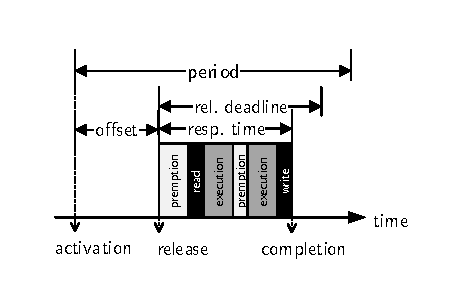
\includegraphics[trim=0.5cm 0.5cm 0.5cm 0.5cm, width=\textwidth]{fig/paper/model_task.pdf}
	\caption{Periodic BET task with release offset.}
	\label{fig:et_task}
\end{subfigure}
%
\hfill
%
\begin{subfigure}[t]{0.45\textwidth}
	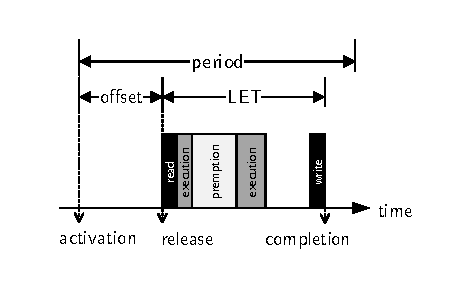
\includegraphics[trim=0.5cm 0.5cm 0.5cm 0.5cm, width=\textwidth]{fig/paper/model_task_let.pdf}
	\caption{LET task with release offset.}
	\label{fig:let_task}
\end{subfigure}
%
\caption{Task model.}
\label{fig:task}
\end{figure}


An \emph{application} is a directed graph $\app = (\taskSet, \dependSet)$, where the set of vertices $\taskSet$ represents the tasks in the application and the set of directed edges $\dependSet$ represents the data-flow dependencies among the tasks. 
An exemplary application is shown in Figure \ref{fig:model_applications}.
\bigskip

\begin{definition}[Cause-effect chain]
A cause-effect chain  
$\cec=(\task[1], \task[2], \ldots, \task[n])$ 
is a finite directed walk in an application $\app$ which is executed on a hardware platform $\platform$.
\end{definition}

\begin{definition}[Instance of a cause-effect chain]
An instance of a cause-effect chain $\cec(\jobSeq)$ 
is a sequence of jobs
$\left(\job[1][j_1], \job[2][j_2], \ldots, \job[n][j_n]\right)$, where each job $\job[{k+1}][j_{k+1}]$ reads data from the predecessor job $\job[k][j_{k}]$.
\end{definition}
%
The concepts of a cause-effect chain and an instance of a cause-effect chain are illustrated in Figure \ref{fig:cec}.
The possible instances of a cause-effect chain can be determined by a data flow analysis, which checks whether a data flow through the sequence of jobs $\job[1][j_1] \job[2][j_2], \ldots, \job[n][j_n]$ is at all possible. 
Please refer to the appendix for details how to perform such a data flow analysis.
\bigskip

The tool \Tool supports time-triggered and LET-triggered cause-effect chains, i.e., cause-effect chains with consists either of only BET tasks or LET tasks.

\begin{figure}
%
\begin{subfigure}[b]{0.5\textwidth}
	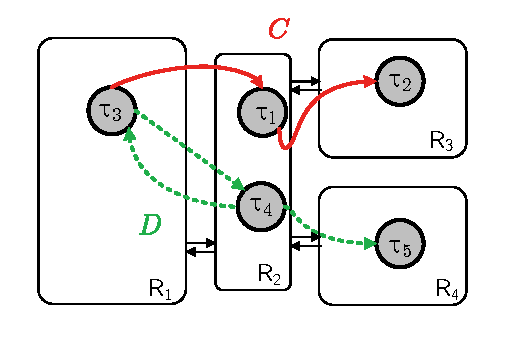
\includegraphics[trim=0.5cm 0.5cm 0.5cm 0.5cm, width=\textwidth]{fig/paper/model_application.pdf}
	\caption{Exemplary cause-effect chains\\ 
	$\cec=(\task[1], \task[2], \task[3])
	= (\taskStd[3], \taskStd[1], \taskStd[2])$  
	and\\ 
	$D=(\task[1][D], \task[2][D], \task[3][D],\task[4][D],\task[5][D])
	= (\taskStd[3], \taskStd[4], \taskStd[3], \taskStd[4], \taskStd[5])$\\
	in an application.}
	\label{fig:model_applications}	
\end{subfigure}
%
\hfill
%
\begin{subfigure}[b]{0.45\textwidth}
	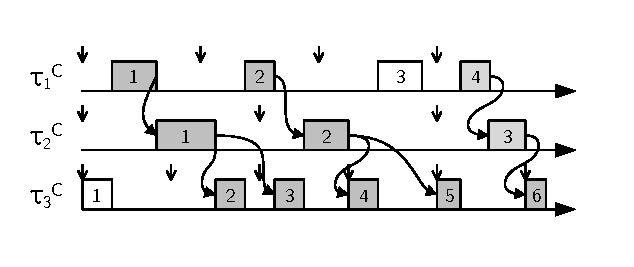
\includegraphics[trim=0.5cm 0.5cm 0.5cm 0.5cm, width=\textwidth]{fig/paper/model_cec_inst.pdf}
	\caption{Exemplary instances of a cause-effect chain  
	$\cec=(\task[\cec_1], \task[2], \task[3])$: \\ 
	$\cec(1,1,2)= \left(\job[1][1], \job[2][1], \job[3][2]\right)$ \\
	$\cec(1,1,3)= \left(\job[1][1], \job[2][1], \job[3][3]\right)$ \\	
	$\cec(2,2,4)= \left(\job[1][2], \job[2][2], \job[3][4]\right)$ \\	
	$\cec(2,2,5)= \left(\job[1][2], \job[2][2], \job[3][5]\right)$ \\	
	$\cec(4,3,6)= \left(\job[1][4], \job[2][3], \job[3][6]\right)$ 
	}
	\label{fig:model_cec}	
\end{subfigure}
%
\caption{Modeling cause-effect chains.}
\label{fig:cec}
\end{figure}

\newpage
\subsubsection{Exemplary Analyzable Systems}
\label{sec:system-model-examples}

\textbf{Application on a single-core ECU} under the following assumptions
\begin{itemize}
	\item Only time-triggered xor LET-triggered cause-effect chains.
	\item Each task meets its deadline or LET.
\end{itemize}

\textbf{Application on a multi-core ECU} under the following assumptions
\begin{itemize}
	\item Only time-triggered xor LET-triggered cause-effect chains.
	\item Each task meets its deadline or LET.
	\item All cores have a common clock, all schedules start simultaneously.
\end{itemize}
%
\textbf{Distributed application on a systems with multiple ECUS connected by data buses and networks} under the following assumptions
	\begin{itemize}
	\item Only time-triggered xor LET-triggered cause-effect chains. 
	\emph{Note that messages can also be modeled as tasks.}
	\item Each task meets its deadline or LET.
	\item All clocks are synchronized, all schedules start simultaneously.
\end{itemize} 
	
\newpage
\subsection{Latencies and Robustness Margins}
\label{sec:outputs}
This section describes which system properties are computed by \Tool. 
For details \emph{how} these properties are computed, please refer to the appendix.


\subsubsection{Maximum End-to-End Latencies}
There are different definitions for end-to-end latencies of cause-effect chains.  
Each definition is relevant in specific contexts, but the most important one is the following:
%
\begin{definition}[End-to-end latency, also: data age]
The end-to-end latency  of an instance of a cause-effect chain, denoted as $\lat{\cec(\jobSeq)}$, is the maximum amount of time that may elapse from the release of the first job $\job[1][j_1]$ to the completion of the last job~$\job[n][j_n]$ in~$\cec(\jobSeq)$.
\end{definition}
%
\begin{definition}[Maximum end-to-end latency]
The maximum end-to-end latency $\latMax$ of a cause-effect chain $\cec$ is an upper bound on the end-to-end latency of any of its instances
\begin{align*}
	\latMax =
	\max_{\cec(\jobSeq) \in \mathcal{C}} 
	\left\{ 
	\lat{\cec(\jobSeq)} 
	\right\}.
\end{align*}
\end{definition}

The maximum end-to-end latency describes how long it can take until fresh input data at the beginning of the cause-effect chain (e.g. a sensor sample) impacts the output of a cause-effect chain (e.g. actuator control value).
This property is important for the reactivity of the system and practical timing requirements often do not  relate to the deadline of tasks but in particular to end-to-end deadlines. 
Tasks deadlines are auxiliary values which emerge in the course of design and implementation.
%
\begin{definition}[End-to-end deadline]
An end-to-end deadline $\eteDeadline$ is the maximum tolerable end-to-end latency of a cause-effect chain $\cec$.
\end{definition}
%


\subsubsection{Robustness Margins}
\label{sec:robustness-margins}
While the maximum end-to-end latency of a cause-effect chain is an important property of the present design, robustness margins indicate to what degree the tasks in a cause-effect chain can be extended in terms of their worst-case response time, resp. LET, without violating timing constraints. 
\bigskip

The tool \Tool computes four different types of robustness margins
\begin{itemize}
	\item Robustness margins for an isolated cause-effect chain  which guarantees the end-to-end deadline
	\item Robustness margins for an isolated cause-effect chain  which guarantees the end-to-end deadline \emph{and} all task deadlines
	\item Robustness margins for a set of possibly dependent cause-effect chains which guarantees all end-to-end deadlines,
	\item Robustness margins for a set of possibly dependent cause-effect chains which guarantees all end-to-end deadlines \emph{and} all task deadlines.			
\end{itemize}
The last type of robustness margin is probably the most important one in practice.


\paragraph{Robustness Margins For an Isolated Cause-Effect Chain} 
This section states the meaning of robustness margins for an isolated cause-effect chain. 
The theorems are based on the paper in the appendix.

\begin{tcolorbox}[colback=black!5!white,colframe=black!75!black, breakable, 
title= \textbf{Theorem}: Robustness test for a single time-triggered cause-effect chain]
Let $\cec = (\task[1], \task[2], \ldots, \task[n])$ be a time-triggered cause-effect chain with the property that each task $\task[k]$ in $\cec$ has a worst-case response time $\wcrt{k}$ satisfying the task deadline $\deadline{k}$. 
Moreover, the cause-effect chain $\cec$ also satisfies its end-to-end deadline $\eteDeadline$.
Let $\disturb[k] \geq 0$ be the increase in the worst-case response time of each task $\task[k]$ in $\cec$ that is caused by a software update.
\smallskip

The time-triggered cause-effect chain $\cec$ still satisfies its end-to-end deadline $\eteDeadline$ under the increase of the worst-case response times of its tasks $\task[k]$ by $\disturb[k]$, if  
\begin{align*}
	& \forall \task[k] \in \cec: \:
	\disturb[k] < \margin{\task[k]} .
\end{align*}	

The time-triggered cause-effect chain $\cec$ still satisfies its end-to-end deadline $\eteDeadline$ \emph{and its task deadlines} under the increase of the worst-case response times of its tasks $\task[k]$ by $\disturb[k]$, if  
\begin{align*}
	& \forall \task[k] \in \cec: \:
	\disturb[k] < 
	\min \{\margin{\task[k]}, \: \deadline{k} - \wcrt{k}\}.
\end{align*}	

\end{tcolorbox}
\smallskip

\begin{tcolorbox}[colback=black!5!white,colframe=black!75!black, breakable, 
title= \textbf{Theorem}: Robustness test for a single LET-triggered cause-effect chain]
Let $\cec = (\task[1], \task[2], \ldots, \task[n])$ be a LET-triggered cause-effect chain with the property that each task $\task[k]$ in $\cec$ satisfies its LET $\Let{k}$. 
Moreover, the cause-effect chain $\cec$ also satisfies its end-to-end deadline $\eteDeadline$.
Let $\disturbLet{k} \geq 0$ be a planned increase of the $\Let{k}$ of a task $\task[k]$.
\smallskip

The LET-triggered cause-effect chain $\cec$ still satisfies its end-to-end deadline $\eteDeadline$ under the increase of the LETs of its tasks $\task[k]$ by $\disturbLet{k}$, if  
\begin{align*}
	& \forall \task[k] \in \cec: \:
	\disturbLet{k} < \margin{\task[k]}. 
\end{align*}	

The LET-triggered cause-effect chain $\cec$ still satisfies its end-to-end deadline $\eteDeadline$ \emph{and its task deadlines} under the increase of the worst-case response times of its tasks $\task[k]$ by $\disturb[k]$, if  
\begin{align*}
	& \forall \task[k] \in \cec: \:
	\disturb[k] < 
	\min \{\margin{\task[k]}, \: \deadline{k} - \Let{k}\}.
\end{align*}	

\end{tcolorbox}
\bigskip

\newpage
\paragraph{Robustness Margins for a Set of Possibly Dependent Cause-Effect Chains}
A task of an application may be part of several cause-effect chains.
Consequently, increasing the worst-case response time (or LET) of this particular task may have an impact on all cause-effect chains that share this task.
We can find new robustness margins $\marginAll{\task[k]}$ (instead of: $\margin{\task[k]}$) which guarantee that \emph{all} cause-effect chains in the application still satisfy their deadlines under a disturbance $\disturb[k]$ resp. $\disturbLet{k}$.
\bigskip

\begin{tcolorbox}[colback=black!5!white,colframe=black!75!black, breakable, 
title= \textbf{Theorem} (Robustness test for time-triggered cause-effect chains)]
Let $\mathcal{S}$ be a set of time-triggered cause-effect chains. 
Each cause-effect chain $\cec = (\task[1], \task[2], \ldots, \task[n])$ in $\mathcal{S}$ has the property that the worst-case response time $\wcrt{k}$ of every task $\task[k]$ in $\cec$ satisfies the task deadline $\deadline{k}$. 
Moreover, each cause-effect chain $\cec$ in $\mathcal{S}$ also satisfies its end-to-end deadline $\eteDeadline$.
%
Let $\disturb[k] \geq 0$ be the increase in the worst-case response time of a task $\task[k]$ in $\taskSet$ that is caused by a software update.
\smallskip

All time-triggered cause-effect chain $\cec$ in $\mathcal{S}$ still satisfy their end-to-end deadlines $\eteDeadline$ under the increase of the worst-case response times of its tasks $\task[k]$ by $\disturb[k]$, if  
\begin{align*}
	& \forall \cec: \forall \task[k] \in \cec: \:
	\disturb[k] < \marginAll{\task[k]}. 
\end{align*}	

All time-triggered cause-effect chain $\cec$ in $\mathcal{S}$ still satisfy their end-to-end deadlines $\eteDeadline$ \emph{and all task deadlines} under the increase of the worst-case response times of its tasks $\task[k]$ by $\disturbLet{k}$, if  
\begin{align*}
	& \forall \task[k] \in \cec: \:
	\disturb[k] < 
	\min \{\marginAll{\task[k]}, \: \deadline{k} - \wcrt{k}\}.
\end{align*}

\end{tcolorbox}
\bigskip

\begin{tcolorbox}[colback=black!5!white,colframe=black!75!black, breakable, 
title= \textbf{Theorem} (Robustness test for LET-triggered cause-effect chains)]
Let $\mathcal{S}$ be a set of LET-triggered cause-effect chains. 
Each cause-effect chain $\cec = (\task[1], \task[2], \ldots, \task[n])$ in $\mathcal{S}$ has the property that every task $\task[k]$ in $\cec$ satisfies its LET $\Let{k}$. 
Moreover, each cause-effect chain $\cec$ in $\mathcal{S}$ also satisfies its end-to-end deadline $\eteDeadline$.
%
Let $\disturbLet{k} \geq 0$ be a planned increase of the $\Let{k}$ of a task $\task[k]$.
\smallskip

All LET-triggered cause-effect chain $\cec$ in $\mathcal{S}$ still satisfy their end-to-end deadlines $\eteDeadline$ under the increase of the LETs of its tasks $\task[k]$ by $\disturbLet{k}$, if  
\begin{align*}
	& \forall \cec: \forall \task[k] \in \cec: \:
	\disturbLet{k} < \marginAll{\task[k]}. 
\end{align*}	

All LET-triggered cause-effect chain $\cec$ in $\mathcal{S}$ still satisfy their end-to-end deadlines $\eteDeadline$ \emph{and all task deadlines} under the increase of the LETs of its tasks $\task[k]$ by $\disturbLet{k}$, if  
\begin{align*}
	& \forall \task[k] \in \cec: \:
	\disturb[k] < 
	\min \{\marginAll{\task[k]}, \: \deadline{k} - \Let{k}\}.
\end{align*}	

\end{tcolorbox}








\newpage
\section{Usability}
This chapter explains how to install and use the tool \Tool.

\subsection{Installation}
This section explains how to install the tool \Tool.
\begin{itemize}[leftmargin=*]
	\item Install a Python Interpreter (version 2.7 or 3).
				You may want to install a distribution (e.g. Python(x,y)) which contains already many useful packages.
	\item The tool \Tool will be delivered in a zipped folder \Code{Toro.zip}. 
				This folder has the following content:
				\begin{itemize}
				\item \textbf{Main script \Code{toro\_main.py}}, 
				\item \textbf{Libraries (pycpa, toro) in the folder \Code{libs}}.
				The libraries under \Code{./libs} are dynamically included. 
				They do not need to be installed unless you want to change their location.
				\item \textbf{Input folder \Code{data}.} Systems to be analyzed can be stored here.
				\end{itemize}
	\item Unzip the zip folder to your preferred destination.	
\end{itemize}


\subsection{Use}
This section gives an overview how to use the tool \Tool.
\begin{itemize}
\item Open a terminal and change to the \Code{/Toro} folder.	
\item The tool \Tool is called via the script \Code{toro\_main.py}.
A path is passed to the script as an argument to specify the location of the system to be analyzed.
It is recommended to store the system to be analyzed in the provided \Code{data} folder.
If several systems are to be analyzed, a subfolder can be created in \Code{data} for each system to be analyzed. 
The folder structure is illustrated in Figure \ref{fig:structure}.
\item An exemplary call of the tool would then look as follows:
\begin{tcolorbox}
\Code{\textbf{user@computer:\textasciitilde/Toro\$} python toro\_main.py ./data}
\end{tcolorbox}
%
\item The tool \Tool then executes, searching for specified systems. 
From the set of found systems, one ore more can interactively be selected for analysis.
Then the same procedure is repeated for each system to be analyzed:
\begin{itemize}
	\item User query to identify the type of system and verify assumptions about the system.
	\item Parsing the csv-files which specify the system (see Section \ref{sec:input-files}.
	\item Calculation of maximum end-to-end latencies and robustness margins.
	\item Generation of diagrams.
	\item Creation of a file containing numerical results.  
	The file is written to the folder in which the analyzed system is specified.
\end{itemize}
\end{itemize}
%
\begin{figure}[t]
		\centering
				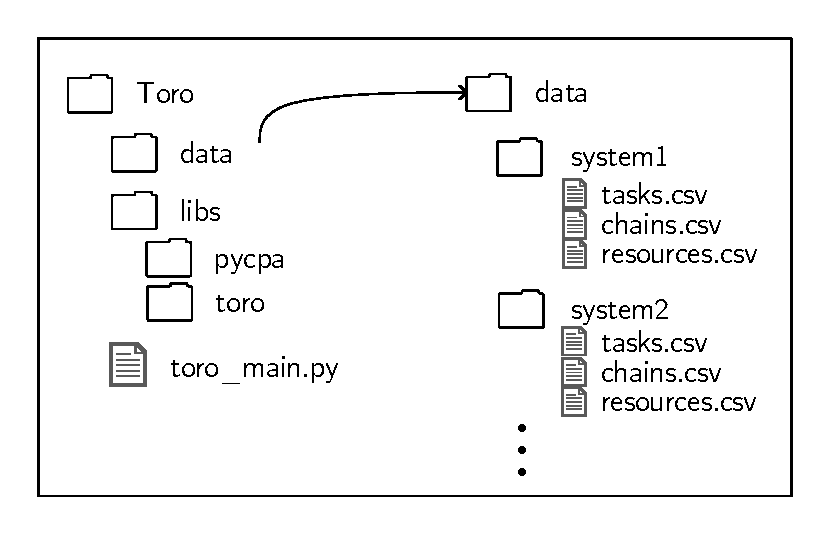
\includegraphics[trim=0.5cm 0.5cm 0.5cm 0.5cm, height=6cm]{fig/structure.pdf}
		\caption{Folder structure}
		\label{fig:structure}
\end{figure}
%


\subsection{Inputs}
\label{sec:input-files}
This section explains how to specify systems that the tool \Tool should analyze.
\bigskip

Firstly, \Tool calls the method \Code{get\_system\_dirs(dir)} and searches the specified folder for systems to be analyzed. 
Each individual system should be encapsulated in a dedicated folder as illustrated in Figure \ref{fig:structure}.
This system folder should contain three semicolon-separated csv-files, namely
\begin{itemize}[itemsep=0pt]
	\item \Code{chains.csv}, 
	\item \Code{resources.csv}, 
	\item \Code{tasks.csv}. 
\end{itemize}
These files can be created in Microsoft Excel, for example, and can then be exported as CSV files.
If \Tool finds more than one system in the specified top-level folder (e.g. \Code{.\\data}), the user can choose from a list which system(s) should be examined. 
An example output would look like this:
\begin{tcolorbox}
\small
{\Code{The following systems have been found:\\
\hspace*{15mm}1: system1\\
\hspace*{15mm}2: system2\\
\hspace*{15mm}2: system3\\
\hspace*{15mm}0: all\\
To select systems enter their ID or a comma-separated list of IDs. For instance, enter 1 to select the first of the listed systems, enter 1,3 to select the first and the third of the listed systems, or enter '0' to select all systems:}}
\end{tcolorbox}

The following sections \ref{sec:input-files-resources}-\ref{sec:input-files-chains} explain the structure of the CSV files. 
Then sections \ref{sec:input-files-bet1}-\ref{sec:input-files-let} demonstrate the three possible types of use cases and which information needs to be filled in.


\subsubsection{Input File 'resources.csv'}
\label{sec:input-files-resources}
The \Code{resources.csv} file describes the execution platform of the system by listing the different resources (CPUs, CAN bus etc.) and the scheduling policy that is applied on each resource. 
%Currently static priority preemptive and static priority non-preemptive scheduling is supported.
The \Code{resources.csv} file should have the following column headers:
\begin{description}
		\item [name] Type: String \hfill \\ 
		Each computing core and each data bus, on which at least one chain task is executed, is represented by a so-called \emph{resource}.   This field specifies the name of the resource.		
		\item [scheduler] Type: String \hfill \\ 
		e.g., \Code{SPPScheduler} or \Code{SPNPScheduler}
\end{description}
\bigskip


\subsubsection{Input File 'tasks.csv'}
\label{sec:input-files-tasks}
The \Code{tasks.csv} file specifies tasks that are executed on the platform, it should have the following column headers:
\begin{description}
		\item [task\_name] Type: String \hfill \\ 
		Unique task ID
		\item [period] Type: Integer \hfill \\ 
		Activation period		
		\item [offset] Type: Integer \hfill \\ 
		Release offset
		\item [priority] Type: Integer \hfill \\ 
		Note that 0 is the highest priority.
		\item [wcet] Type: Integer \hfill \\ 
		Worst Case Execution Time		
		\item [resource] Type: String \hfill \\ 
		Resource that services the task. 
		The name should match a resource from file \Code{pycpa\_resources.csv}.
		\item [bcrt] Type: Integer \hfill \\ 
		Best Case Response Time		
		\item [wcrt] Type: Integer \hfill \\ 
		Worst Case Response Time
		\item [let] Typ: Integer \hfill \\ 
		Logical Execution Time 
\end{description}
\bigskip


\subsubsection{Input File 'chains.csv'}
\label{sec:input-files-chains}
The \Code{chains.csv} file specifies which tasks are part of each cause-effect chain; it should have the following column headers:
\begin{description}
		\item [chain\_name] Type: String \hfill \\ 
		Unique cause-effect chain ID
		\item [e2e\_deadline] Type: Integer \hfill \\ 
		End-to-end deadline 		
		\item [members] Type: String \hfill \\ 
		The member tasks must be listed in correct order and the task names must match those in the task definitions. The list of member tasks comprises as many cells in a row as needed.
\end{description}



\newpage
\subsubsection{Use Case 1:Cause-effect chains with BET tasks, WCRT for each chain task known}
\label{sec:input-files-bet1}

\begin{tcolorbox}
\begin{itemize}[leftmargin=*, itemsep=0pt]
	\item applicable to many systems
	\item the name, period, offset, WCRT of every task in a cause-effect chain must be known
\end{itemize}
\end{tcolorbox}
\bigskip

For \emph{Use Case 1} given that
\begin{itemize}[leftmargin=*, itemsep=0pt]
	\item all clocks in the system are synchronized,
	\item all tasks in the cause-effect chains are BET tasks,
	\item task deadlines are implicit,
\end{itemize}
(which is checked in an interactive user query), 
it is sufficient to specify the following details of the entire systems.
An example system of type \emph{'Use Case 1'} is depicted in Figure \ref{fig:use-case-1}.

For the example system, the file \Code{resources.csv} would contain:
\begin{center}
	\begin{tabular}{|l|l|} \hline
		\textbf{name} & \textbf{scheduler} \\ \hline
		unknown & unknown \\ \hline
	\end{tabular}
\end{center}
With regard to the tasks that are part of the cause-effect chains to be analyzed, we have in \Code{tasks.csv} 
\begin{center}
	\begin{tabular}{|l|l|l|l|l|l|l|l|l|} \hline
		  \textbf{task\_name}  
		& \textbf{period} 
		& \textbf{offset} 
		& \textbf{priority}
		& \textbf{wcet}
		& \textbf{resource} 
		& \textbf{bcrt}		
		& \textbf{wcrt}
		& \textbf{let} \\ \hline
	\end{tabular}
\end{center}
Note that a number of fields in \Code{resources.csv} and \Code{tasks.csv} can be left empty or declared as 'unknown' because the WCRTs are already available and do not need to be computed from these parameters.
\bigskip

The cause-effect chains in \Code{chains.csv} are specified by
\begin{center}
	\begin{tabular}{|l|l|l|l|l|} \hline
		\textbf{chain\_name} 
		& \textbf{e2e\_deadline}
		& \multicolumn{3}{|l|}{\textbf{members}} \\ \hline
	\end{tabular}
\end{center}
%
\begin{figure}[h!]
	\centering
		\includegraphics[width=0.7\textwidth,page=2]{fig/example_input.pdf}
	\caption{Use case 1; relevant parts of the system for the analysis are marked in color.}
	\label{fig:use-case-1}
\end{figure}



\newpage
\subsubsection{Use Case 2: Cause-effect chains with BET tasks,\\ WCRT of each chain task computable}
\label{sec:input-files-bet2}

\begin{tcolorbox}
\begin{itemize}[leftmargin=*, itemsep=0pt]
	\item only applicable to systems with \ac{spp} und \ac{spnp} scheduling
	\item not only tasks that are part of cause-effect chains must be specified but also the entire background load with all parameters
\end{itemize}
\end{tcolorbox}

For \emph{Use Case 2} given that
\begin{itemize}[leftmargin=*, itemsep=0pt]
	\item all clocks in the system are synchronized,
	\item ALL tasks are BET tasks (not only those in the listed cause-effect chains),
	\item task deadlines are implicit,	
	\item ALL tasks in the system must be known with their parameters,
	\item ALL resources must be known with their scheduling algorithms (SPP or SPNP) and the task-to-resource mapping,
\end{itemize}
(which is checked in an interactive user query), 
it is sufficient to specify the following details of the entire systems.
An example system of type \emph{'Use Case 2'} is depicted in Figure \ref{fig:use-case-2}.
For the example system, the file \Code{resources.csv} would contain:

\begin{center}
\small
	\begin{tabular}{|l|l|} \hline
		\textbf{Name} & \textbf{Scheduler} \\ \hline	
	\end{tabular}
\end{center}

With regard to the tasks that are part of the cause-effect chains to be analyzed, we have not only the chain tasks but also the tasks of the background load with all parameters required to compute the WCRTs.
\begin{center}
	\begin{tabular}{|l|l|l|l|l|l|l|l|l|} \hline
		  \textbf{task\_name}  
		& \textbf{period} 
		& \textbf{offset} 
		& \textbf{priority}
		& \textbf{wcet}
		& \textbf{resource} 
		& \textbf{bcrt}		
		& \textbf{wcrt}
		& \textbf{let} \\ \hline
	\end{tabular}
\end{center}

The cause-effect chains are specified again by
\begin{center}
	\begin{tabular}{|l|l|l|l|l|} \hline
		\textbf{chain\_name} 
		& \textbf{e2e\_deadline}
		& \multicolumn{3}{|l|}{\textbf{members}} \\ \hline
	\end{tabular}
\end{center}
%
\begin{figure}[h!]
	\centering
		\includegraphics[width=0.7\textwidth,page=3, trim = 0.5cm 0.5cm 0.5cm 0.5cm]{fig/example_input.pdf}
	\caption{Use case 2; relevant parts of the system for the analysis are marked in color}
	\label{fig:use-case-2}
\end{figure}


\newpage
\subsubsection{Use Case 3: Cause-effect chains with LET tasks, LET for each chain task known}
\label{sec:input-files-let}
%

\begin{tcolorbox}
\begin{itemize}[leftmargin=*, itemsep=0pt]
	\item applicable to LET systems
\end{itemize}
\end{tcolorbox}
\bigskip

For \emph{Use Case 3} given that
\begin{itemize}[leftmargin=*, itemsep=0pt]
	\item all clocks in the system are synchronized,
	\item all tasks in the cause-effect chains are LET tasks,
	\item all LET tasks have implicit deadlines,	
\end{itemize}
(which is checked in an interactive user query), 
it is sufficient to specify the following details of the entire systems.
An example system of type \emph{'Use Case 3'} is depicted in Figure \ref{fig:use-case-3}.

For the example system, the file \Code{resources.csv} would contain:
\begin{center}
	\begin{tabular}{|l|l|} \hline
		\textbf{name} & \textbf{scheduler} \\ \hline
		unknown & unknown \\ \hline
	\end{tabular}
\end{center}
With regard to the tasks that are part of the cause-effect chains to be analyzed, we have in \Code{tasks.csv} 
\begin{center}
	\begin{tabular}{|l|l|l|l|l|l|l|l|l|} \hline
		  \textbf{task\_name}  
		& \textbf{period} 
		& \textbf{offset} 
		& \textbf{priority}
		& \textbf{wcet}
		& \textbf{resource} 
		& \textbf{bcrt}		
		& \textbf{wcrt}
		& \textbf{let} \\ \hline
	\end{tabular}
\end{center}

The cause-effect chains are specified by
\begin{center}
	\begin{tabular}{|l|l|l|l|l|} \hline
		\textbf{chain\_name} 
		& \textbf{e2e\_deadline}
		& \multicolumn{3}{|l|}{\textbf{members}} \\ \hline	
	\end{tabular}
\end{center}
%
\begin{figure}[h!]
	\centering
		\includegraphics[width=0.7\textwidth,page=2]{fig/example_input.pdf}
	\caption{Use case 3; relevant parts of the system for the analysis are marked in color.}
	\label{fig:use-case-3}
\end{figure}


\newpage
\subsection{Outputs}
\label{sec:outputs}
Outputs are written into the folder of the specified system.

\subsubsection{Log File}
The numberical results are written to the text file 
\Code{RESULTS_LOG.txt}.

\subsubsection{Interval Diagram}
%
\begin{figure}
		\centering
		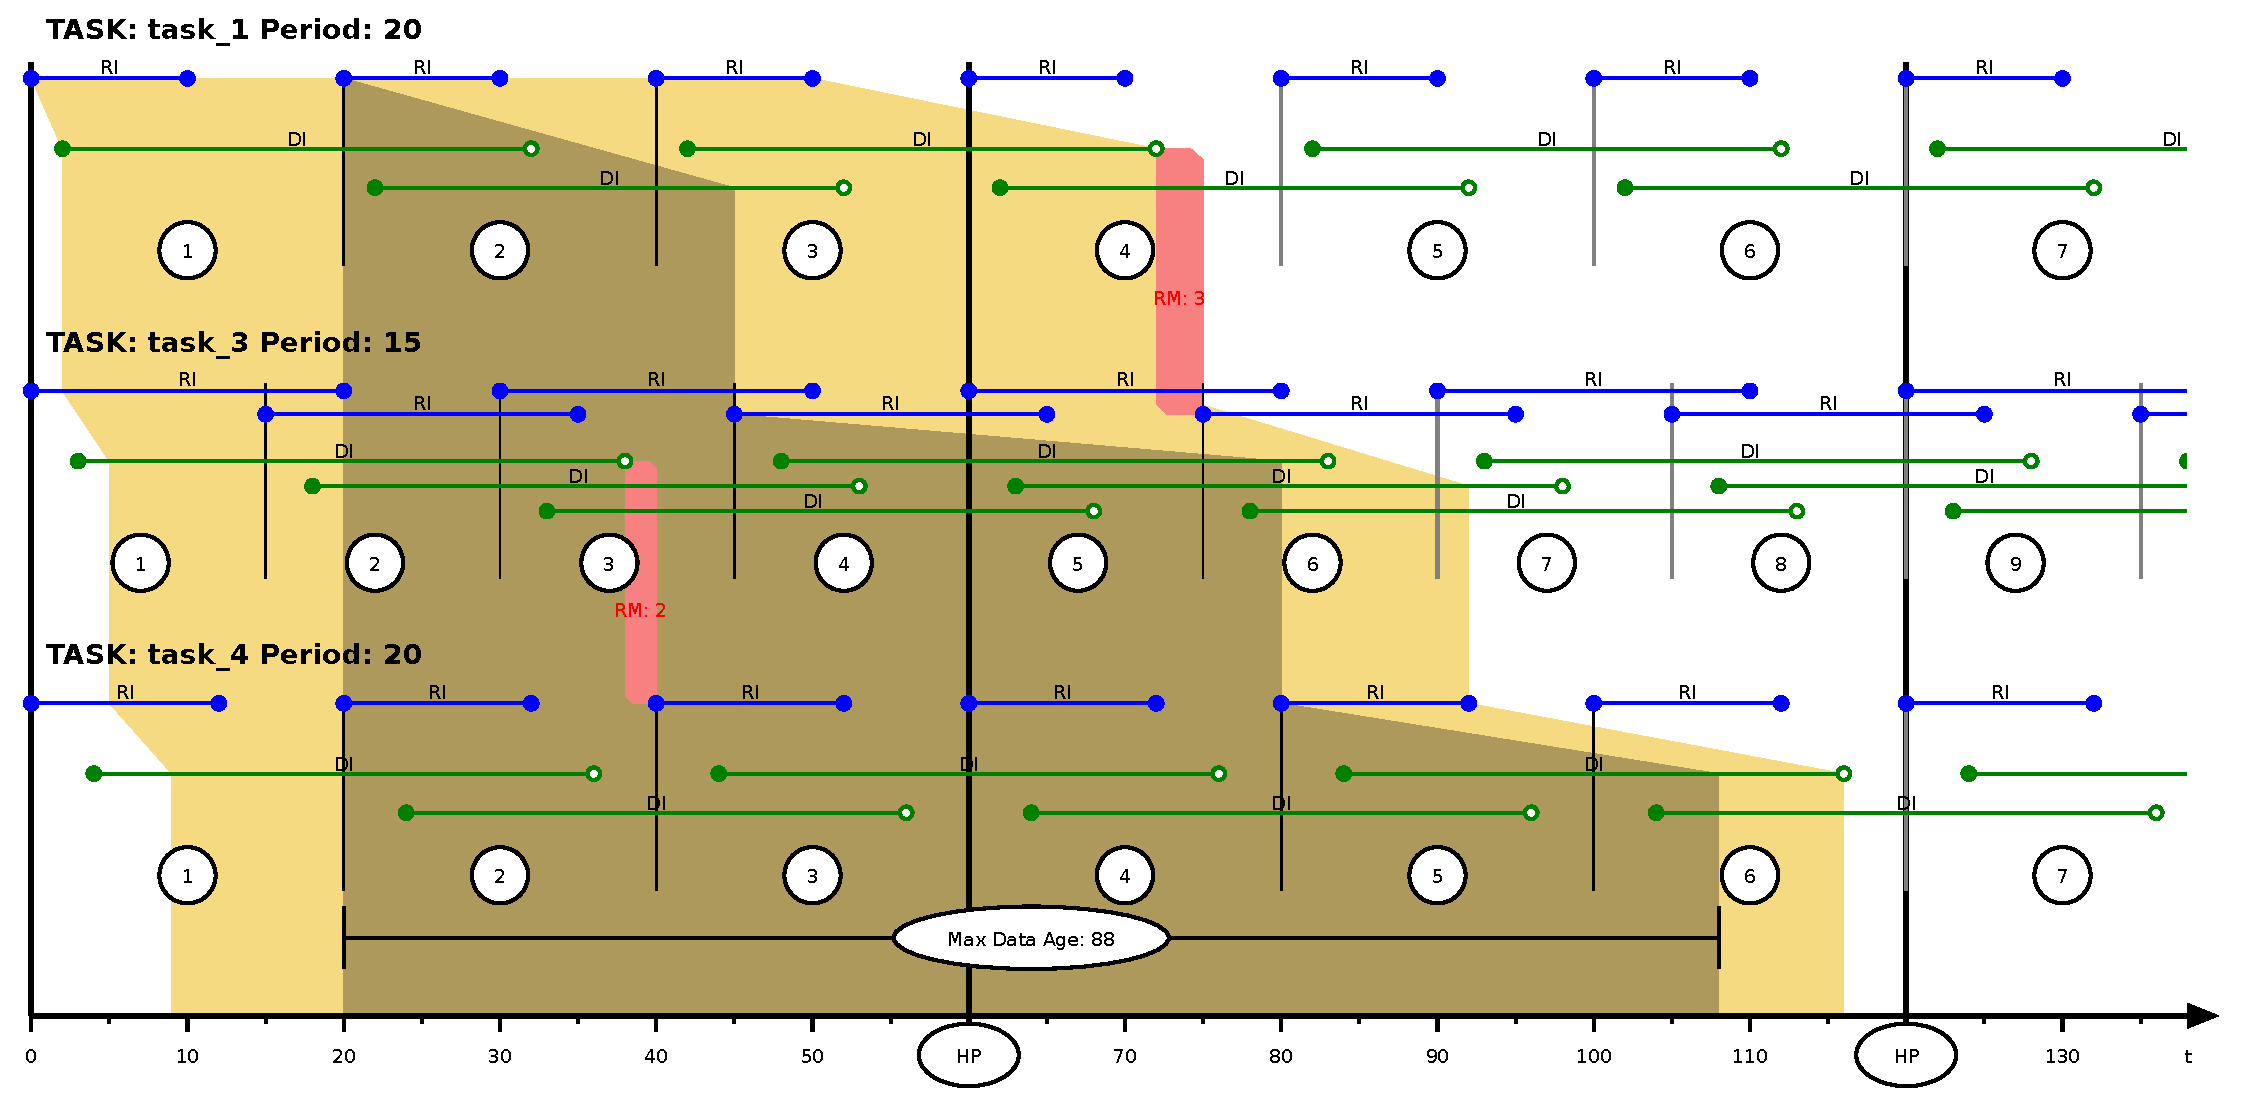
\includegraphics[width=415pt]{fig/intervalls.pdf}
		\caption{Interval diagram.}
		\label{fig:interval_diagram}
\end{figure}
%
In the interval diagram, the individual jobs are represented as numbered circles. 
The blue-marked read intervals represent the earliest possible to latest possible time, when a job can read data. 
The green-marked data intervals bound the period of time in which the output data of a job is available to other jobs.
The short vertical lines stand for the period of a task.
The long vertical lines show the hyper period (HP).
\smallskip

The yellow area covers all instances of the cause-effect chain which are relevant for the computation of the maximum end-to-end latency and the robustness margins. \\
The dark area highlights one instance of a cause-effect chains which actually has the maximum end-to-end latency. \\
The red areas illustrate some selected robustness margins, which are valid for the isolated cause-effect chain (not for the set of specified cause-effect chains in \Code{chains.csv}.


\newpage
\subsubsection{Reachability Graph}
%
\begin{figure}[H]
		\centering
		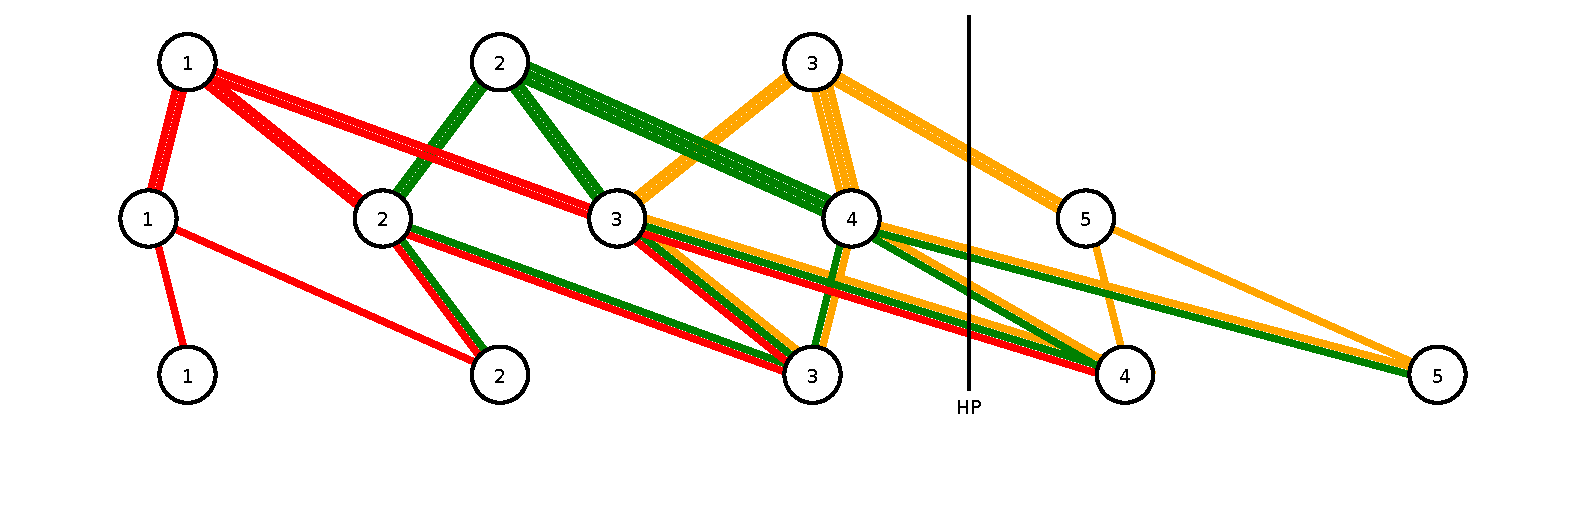
\includegraphics[width=400pt]{fig/tree.pdf}
		\caption{Reachability graph}
		\label{fig:reachability}
\end{figure}
%
The reachability graph results from the overlap of read intervals and data intervals of jobs (data flow analysis). 
In the reachability graph, all possible paths of starting in from the first hyperperiod are represented.
These paths are required for the computation of the maximum end-to-end latency and the robustness margins. 
The colored marking of the individual paths makes it easy to recognize where a path begins and ends. The numbers stand for the respective job number. 
    

\newpage
\subsubsection{Overview Graph}
The overview graph represents the specified cause-effect chains as a tasks with data flow dependencies.
Moreover, it lists the computed maximum end-to-end latencies for each cause-effect chain.
Finally, it indicates the robustness margins for the isolated chains and in the presence of all chains.
%
\begin{figure}[H]
  \centering
  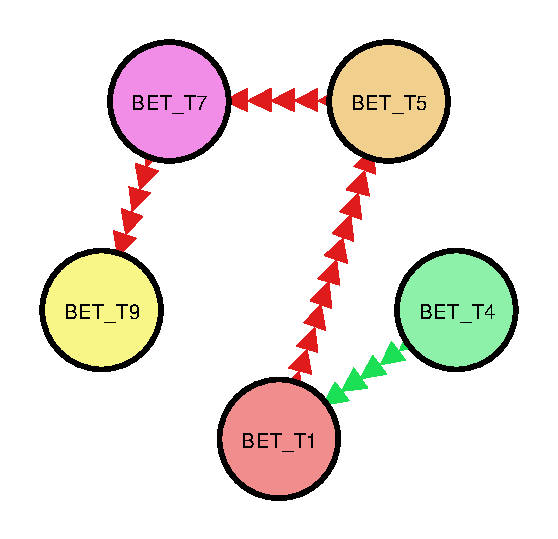
\includegraphics[width=400pt]{fig/results.pdf}
  \caption{Summarizing diagram.}
  \label{fig:summ_diagram}
\end{figure}



\newpage
\section{Internals}

The tool \Tool relies on the Python packages
\begin{itemize}[itemsep=0pt]
	\item \Code{toro}
	\item \Code{pycpa}
\end{itemize}
and the main script
\begin{itemize}[itemsep=0pt]
	\item \Code{toro\_main.py}
\end{itemize}
Details about the \Code{pycpa} package can be found in the online documentation at \url{https://pycpa.readthedocs.io}.
The other two components are discussed in more detail in the following sections \ref{sec:script} and \ref{sec:toro_lib}.
    
\subsection{User Script}
\label{sec:script}
The main script \Code{toro\_main.py} consists of two methods (cf. Figure \ref{fig:toro_internals}):

\paragraph{get\_system\_dirs(dir)}
The script \Code{toro\_main.py} starts with the main method and passes the call parameter (folder path) to the \Code{get\_system\_dirs(dir)} method. \\
The method \Code{get\_system\_dirs(dir)} searches for existing systems under the specified path. 
If more than one system is found, the user can choose from a list which systems should to be analyzed. 

\paragraph{perform\_analysis(dir)}
The method \Code{perform\_analysis(dir)} 
\begin{itemize}[itemsep=0pt]
	\item starts a user query to identify the type of system and verify assumptions about the system,
	\item parses the csv-files which specify the system,
	\item calculates the maximum end-to-end latencies and robustness margins,
	\item generates of diagrams,
	\item logs the numerical results (\Code{RESULTS\_LOG.txt}), 
\end{itemize}
for each of the selected systems.
 %
\begin{figure}[H]
		\centering
		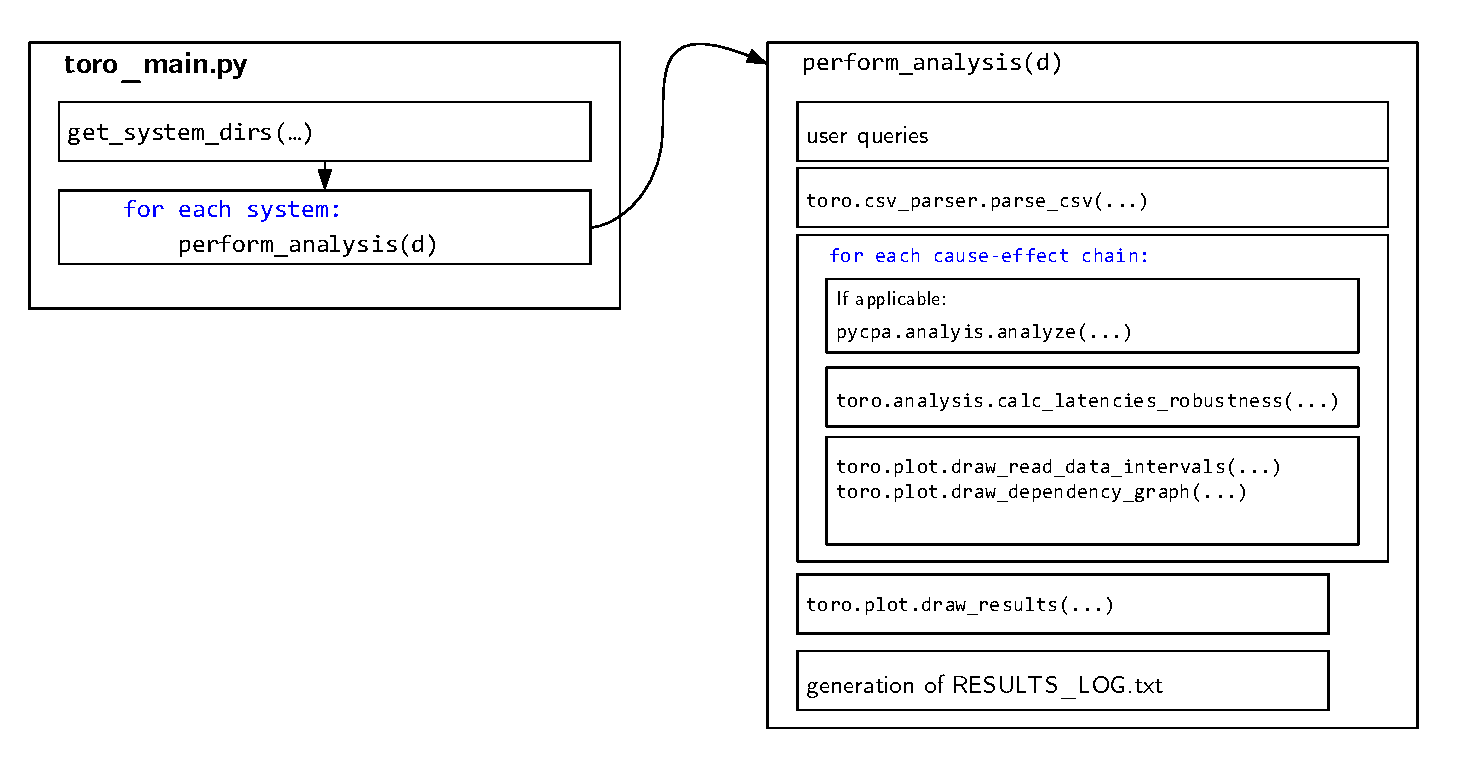
\includegraphics[width=\textwidth]{fig/toro_architecture.pdf}
		\caption{Internals of the main script \Code{toro\_main.py}}
		\label{fig:toro_internals}
\end{figure}

 
\subsection{Toro Package}
\label{sec:toro_lib}
    
This section describes the modules in the package \Code{toro}.

\paragraph{toro.model}
This module defines the data structures required within the software. 
It is an extension of the module of the same name from the \Code{pycpa} package.

\paragraph{toro.analysis}
This module contains the \Code{calc\_latencies\_robustness} class.
When an object of this class is initialized and a chain is passed as an argument, then the maximum latency and the robustness margins for each task are computed.

\paragraph{toro.csv\_parser}
This module reads the CSV-files from the specified folder and transfers them into the software's internal data structure. 
If files are not available or data is not properly defined, an error message is issued. 
The parser is called via the \Code{prase\_csv} class, which requires the folder path of the system to be analyzed as argument.

\paragraph{toro.plot}
The module plots creates graphical representations of the analysis results; the three different types of graphs have been discussed in the section \ref{sec:outputs}.
The module consists of several classes, each is designed for one of the graphical output formats. 

\begin{description}
\item[\Code{image}] 
The \Code{image} class provides the basic functions to draw circles, lines, text and other elements in an SVG image.  
%
\item[\Code{draw\_read\_data\_intervals}] 
This class draws the read and data intervals of jobs in a representative time window on the basis of the analysis results. 
In addition, the computed properties -- maxmimum end-to-end latency and the robustness margins for the isolated chain -- can be drawn using the options "all", "none", "first" and "last". 
A further option is to include the "Dependency Polygon":
\begin{itemize}
		\item max\_data\_age = all | first | last | none
		\item robustness\_margin = all | first | last | none
		\item dependency\_polygon = True | False.
\end{itemize}    
												
\item[\Code{draw\_dependency\_graph}] 
The reachability graph illustrates possible instances of a cause-effect chain. As the call parameter are the analysis results required.
%
\item[\Code{draw\_results}] 
The relevant results of all tasks and cause-effect chains of a system are displayed in an overview graph. 
Chains and tasks are used as call parameters. 
%
\end{description}
\newpage
\section{Internals}

The tool \Tool relies on the Python packages
\begin{itemize}[itemsep=0pt]
	\item \Code{toro}
	\item \Code{pycpa}
\end{itemize}
and the main script
\begin{itemize}[itemsep=0pt]
	\item \Code{toro\_main.py}
\end{itemize}
Details about the \Code{pycpa} package can be found in the online documentation at \url{https://pycpa.readthedocs.io}.
The other two components are discussed in more detail in the following sections \ref{sec:script} and \ref{sec:toro_lib}.
    
\subsection{User Script}
\label{sec:script}
The main script \Code{toro\_main.py} consists of two methods (cf. Figure \ref{fig:toro_internals}):

\paragraph{get\_system\_dirs(dir)}
The script \Code{toro\_main.py} starts with the main method and passes the call parameter (folder path) to the \Code{get\_system\_dirs(dir)} method. \\
The method \Code{get\_system\_dirs(dir)} searches for existing systems under the specified path. 
If more than one system is found, the user can choose from a list which systems should to be analyzed. 

\paragraph{perform\_analysis(dir)}
The method \Code{perform\_analysis(dir)} 
\begin{itemize}[itemsep=0pt]
	\item starts a user query to identify the type of system and verify assumptions about the system,
	\item parses the csv-files which specify the system,
	\item calculates the maximum end-to-end latencies and robustness margins,
	\item generates of diagrams,
	\item logs the numerical results (\Code{RESULTS\_LOG.txt}), 
\end{itemize}
for each of the selected systems.
 %
\begin{figure}[H]
		\centering
		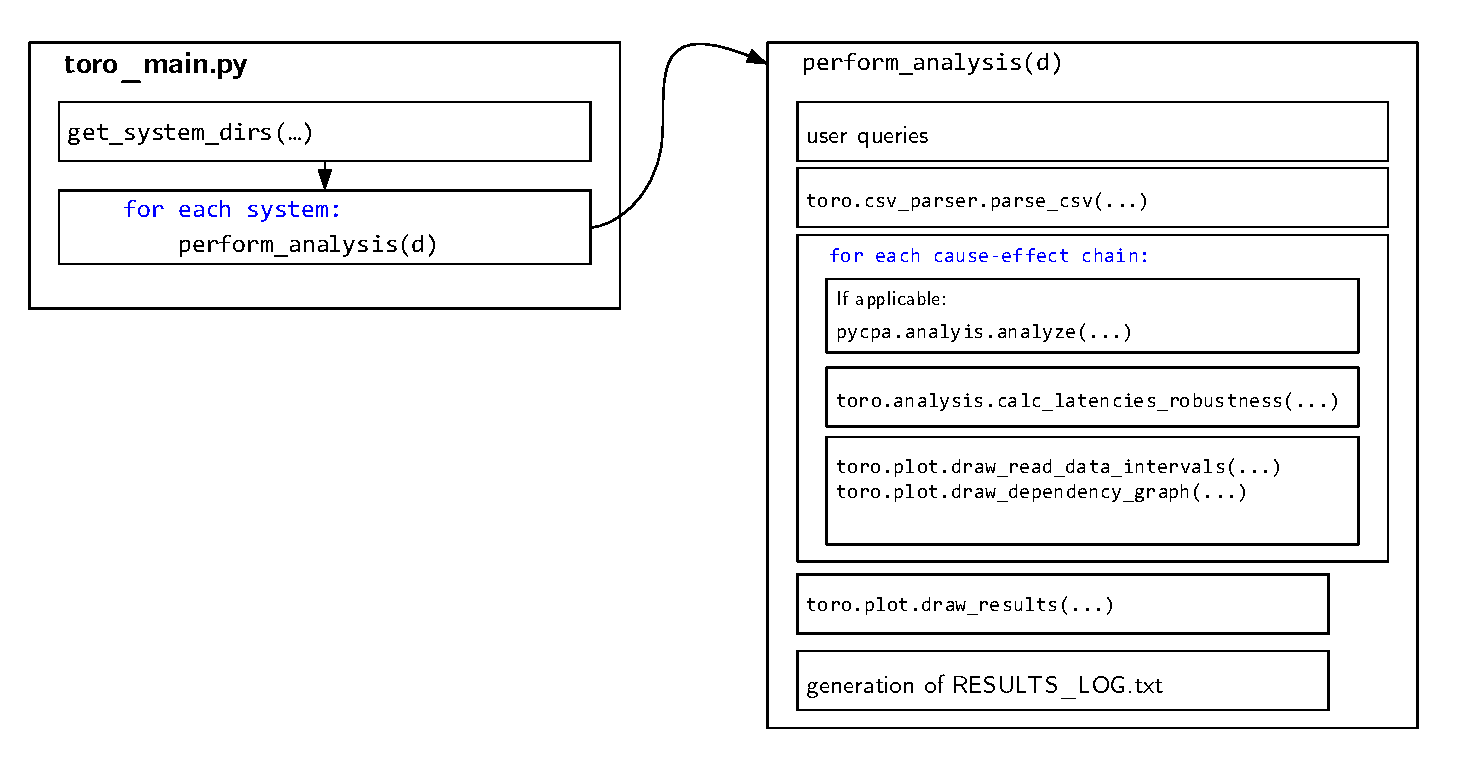
\includegraphics[width=\textwidth]{fig/toro_architecture.pdf}
		\caption{Internals of the main script \Code{toro\_main.py}}
		\label{fig:toro_internals}
\end{figure}

 
\subsection{Toro Package}
\label{sec:toro_lib}
    
This section describes the modules in the package \Code{toro}.

\paragraph{toro.model}
This module defines the data structures required within the software. 
It is an extension of the module of the same name from the \Code{pycpa} package.

\paragraph{toro.analysis}
This module contains the \Code{calc\_latencies\_robustness} class.
When an object of this class is initialized and a chain is passed as an argument, then the maximum latency and the robustness margins for each task are computed.

\paragraph{toro.csv\_parser}
This module reads the CSV-files from the specified folder and transfers them into the software's internal data structure. 
If files are not available or data is not properly defined, an error message is issued. 
The parser is called via the \Code{prase\_csv} class, which requires the folder path of the system to be analyzed as argument.

\paragraph{toro.plot}
The module plots creates graphical representations of the analysis results; the three different types of graphs have been discussed in the section \ref{sec:outputs}.
The module consists of several classes, each is designed for one of the graphical output formats. 

\begin{description}
\item[\Code{image}] 
The \Code{image} class provides the basic functions to draw circles, lines, text and other elements in an SVG image.  
%
\item[\Code{draw\_read\_data\_intervals}] 
This class draws the read and data intervals of jobs in a representative time window on the basis of the analysis results. 
In addition, the computed properties -- maxmimum end-to-end latency and the robustness margins for the isolated chain -- can be drawn using the options "all", "none", "first" and "last". 
A further option is to include the "Dependency Polygon":
\begin{itemize}
		\item max\_data\_age = all | first | last | none
		\item robustness\_margin = all | first | last | none
		\item dependency\_polygon = True | False.
\end{itemize}    
												
\item[\Code{draw\_dependency\_graph}] 
The reachability graph illustrates possible instances of a cause-effect chain. As the call parameter are the analysis results required.
%
\item[\Code{draw\_results}] 
The relevant results of all tasks and cause-effect chains of a system are displayed in an overview graph. 
Chains and tasks are used as call parameters. 
%
\end{description}
\newpage
\appendix
\section{APPENDIX: The Theory Behind Toro\\ \emph{Conference Article in Preparation for ECRTS'20}}
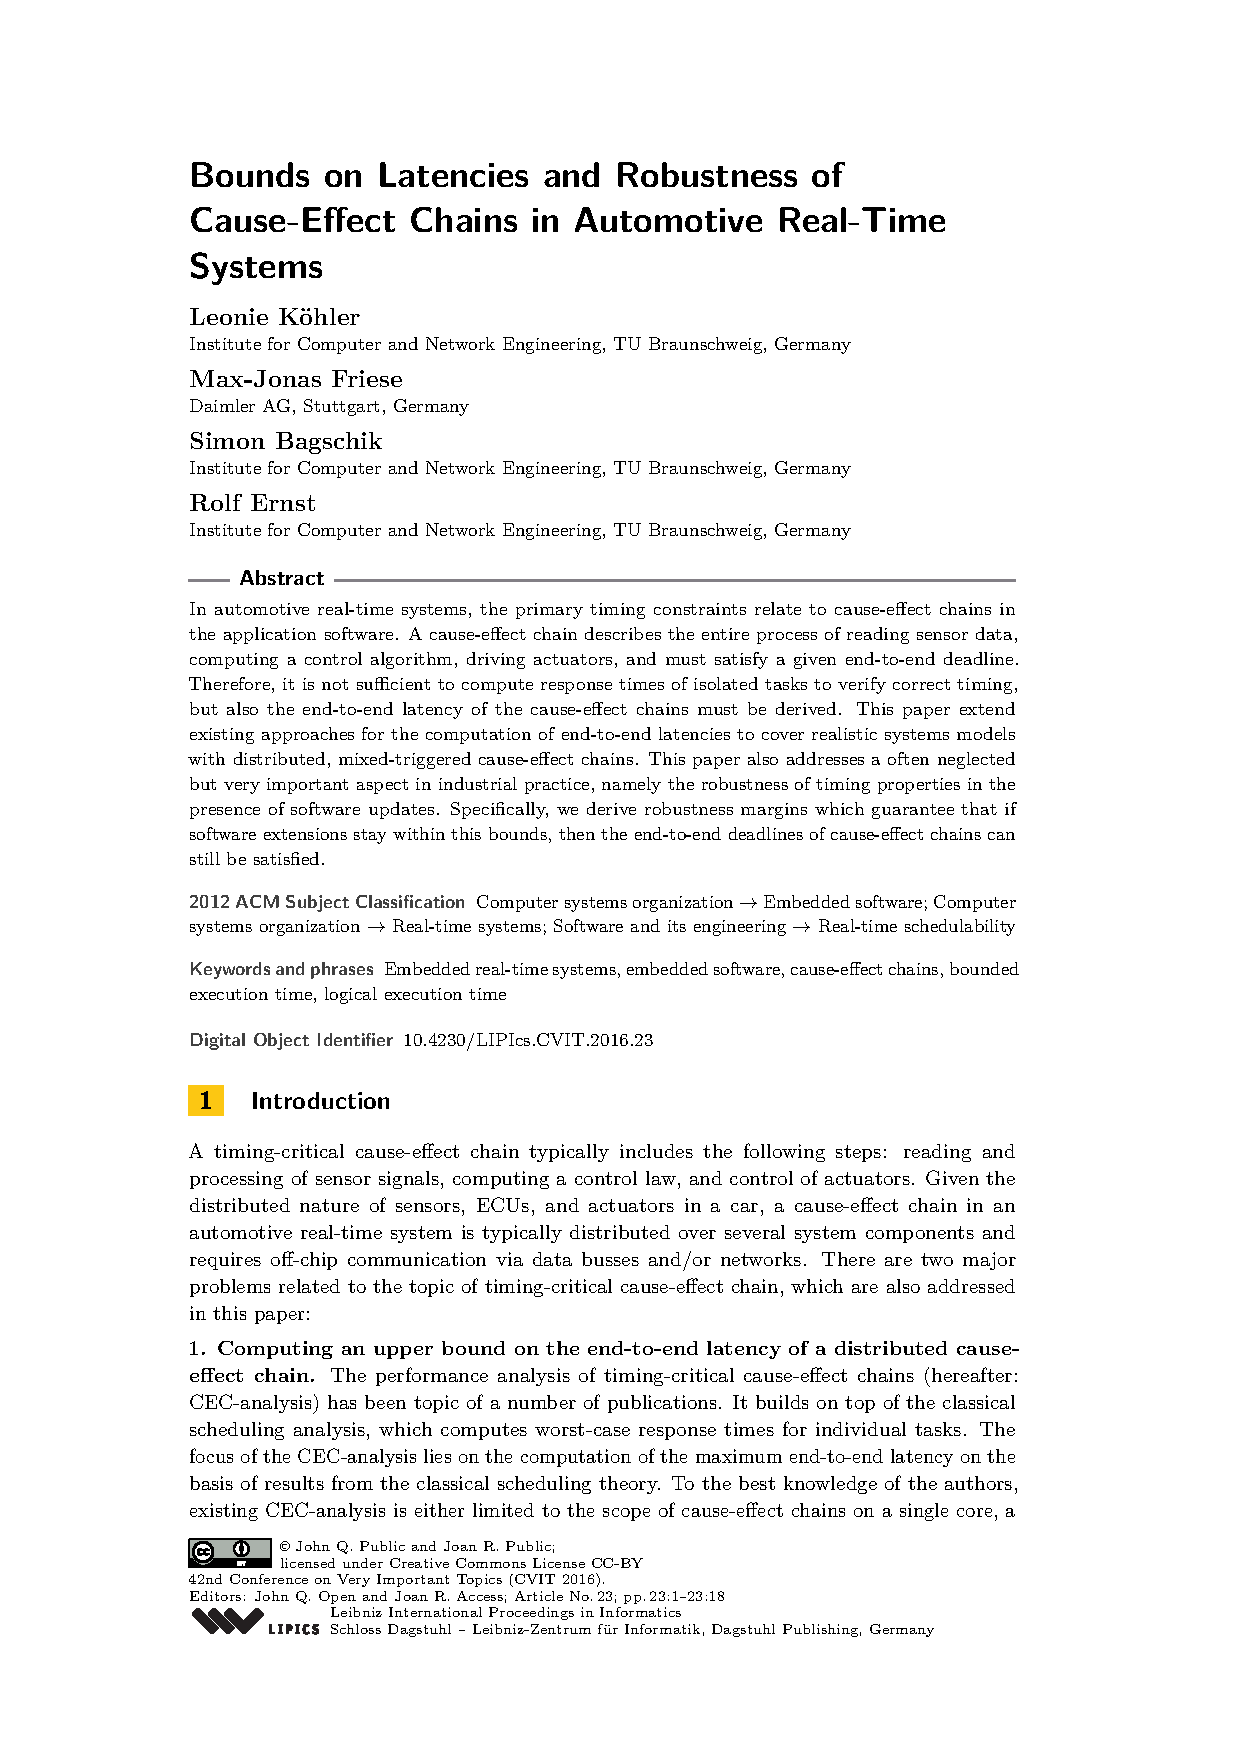
\includepdf[pages=-]{text/ecrts2020_v1.pdf}


\end{document}
